
\chapter{Audio file formats and steganography techniques}

\begin{multicols*}{2}
\section{Introduction}
Sound is the result of a vibration created by a phenomenon that propagates through a transmission environment, ending up getting interpreted by our brain. However since this process happens in the physical world it is entirely analog so it would be impossible to store it on modern day devices which can only understand digital formats. Luckily the fast evolution of computers also brought conversion techniques in order to switch between analog sounds and digital sounds seamlessly, without any noticeable loss to the human ear. Using these methods we have gained the ability to store audio files in a digital format so it was only logical that several different file formats will be created to fit our needs. In this chapter we will discuss in greater detail about how the analog data is actually stored in the digital format and what are the most common extensions used for storing digital audio files.

We mentioned earlier that it is impossible to store analog signals in a digital environment. The solution to this problem is to convert the audio signal which can be represented as a continuous-time function into a discrete-time function using a process called sampling. 

\begin{figure}[H]
    \centering
    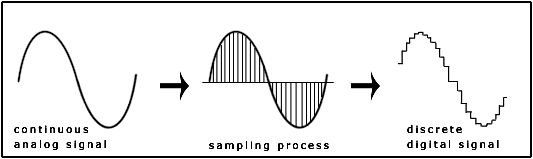
\includegraphics[width=7.7cm,keepaspectratio]{pics/Sampling-of-audio-signal.png}
    \caption{Converting a continuous signal into a discrete one\cite{real_time_audio_steganography}.}
    \label{sampling-graphic-example}
\end{figure}

The sampling process can be observed in figure \ref{sampling-graphic-example}. We can now introduce some new terms that we will use throughout the rest of the chapter:
\begin{itemize}
	\item \textbf{Sampling rate} is the number of samples taken per second, or in other terms, how many discrete values we store for each second of the audio signal. The measurement unit for sampling rate is Hertz (Hz for short) and some of the most common values are 44100, 48000 and some of their multiples.
	\item \textbf{Bit depth} is the number of bits used to store a single sample after having it converted to a discrete value. The most common bit depths are 8, 16, and 24 which allow for 256, 65536, and 16777216 different values. 
	\item \textbf{Audio channel} is the term used to describe the sequence of bytes that represent sampled audio signals. An audio file can have multiple channels to better simulate the sound accuracy and origin in a limited environment. Files with one audio channel are called mono, with two they become stereo and any more channels makes them surround. However, no matter the number of channels, usually all of them are equal in length and the samples from each channel are played simultaneously.
\end{itemize}

In the steganography field, the most common configuration that accepts alterations to the sampled data without losing any noticeable quality is a sampling rate of 44.1kHz with a bit depth of 16 and any number of audio channels, so this the ideal format that we will use throughout the rest of the chapter. The reason why this configuration is favored so much is because of the popularity that came with the invention of CDs and MP3s which used it as a default. Furthermore, any changes made to the sampled data are usually small enough that they will not be noticeable according to the Nyquist-Shannon sampling theorem \cite{Shannon1949}, which is used to compute the condition such that the conversion from a continuous signal to a discrete one will capture all the relevant information. Using the aforementioned theorem and armed with the knowledge that the human physiology enables us to hear audio signals ranging from 20Hz to 20kHz, we can see why the 44.1kHz sampling rate is ideal in audio steganography.

\section{Additional techniques used in audio steganography}
\subsection{Frequency domain steganography}
So far in this thesis we have talked about what can only be classified as spatial domain steganography, like how a pixel of an image is composed of bytes and that altering those byte values in a smart way allows for message embedding or how we can use the file specifications to our advantage and hide information in the file metadata or after the offset where all renderer programs will stop parsing. All of the previous examples deal ony with the spatial domain of the format because they work on the raw bytes and consider each of them to be completely individual and self-sustaining entities that can be altered for steganographic purposes. However, there is another domain that works differently than the spatial one and it is called the frequency domain. In this domain the final representation of the stored data is done by combining the entire range of frequencies into the equivalent signal, usually by using a transform function, the most common being the Fourier transform. The advantage of the frequency domain is that it helps split a signal of any type into clear and distinct sinusoids that are easier to perform complex tasks on. 

In figure \ref{time_vs_frequency_comparison} we can see the differences between the time domain and the frequency domain: the former evolves over time and is highly irregular in most cases(in real world there will never be a perfect sinusoidal signal and will be more similar to the last example), while the latter is easier to manipulate and identify, and through the aforementioned transform functions can be converted back into the time domain.
\begin{figure}[H]
    \centering
    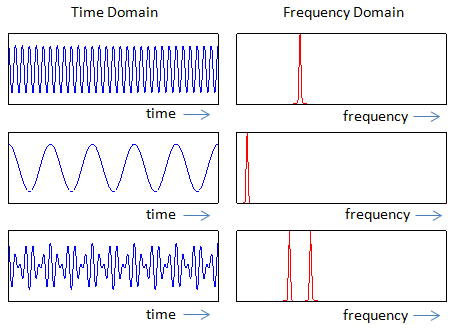
\includegraphics[width=7.7cm,keepaspectratio]{pics/audio_chapter/time_vs_frequency_domains.png}
    \caption{Time domain vs. frequency domain.}
    \label{time_vs_frequency_comparison}
\end{figure}

In the digital images world, the frequency domain is used to know by how much pixels variate from one another, in other words, the rate with which the pixels change. The most common format used for images that takes advantage of the frequency domain is JPEG, but since it is the only known format which uses sinusoids when rendering the image, the authors chose not to include it since the steganographic surface was somewhat limited. However, in the digital audio world every sound will eventually become an analog signal before reaching our ears so it is more common to see algorithms developed specifically for this format that involve altering the sinusoids to our advantage.

For example, we have the technique described in the article Frequency Domain Steganography by Ganier et al.\cite{ganier_hollman_rosser_swanson} where they showcase the most basic way of embedding an audio file within another audio file: since both files have audio signals that are stored as frequencies, it is possible to "compress" the signals so that they only occupy a very specific frequency range and hide the message within the inaudible frequencies of the carrier, a much trivial task when not working in the time domain. This method takes advantage of the human physiology we mentioned earlier and achieves a high rate of success. Similar work has been done by Westfeld et al. \cite{dsss_sstv} where they took the audio signal generated by the Slow Scan Television(SSTV) and embedded it into another carrier audio signal without any audible noise being generated that could alert intruders. On the more technical and software side of things there are applications such as Audacity that can integrate plugins written in a language called Nyquist that are specifically designed for frequency encoding secret messages, along with Matlab implementations of the aforementioned papers and many more.

Furthermore, there is also the option of steganography done within the spectrogram of a signal. A spectrogram is the visual represention of the entire spectrum of the frequencies as it evolves over time, basically getting the frequency domain and reintroducing the time axis into it. It is by far the most common place of hiding messages because it has been popularized by Capture the Flag competitions as entry level challengs and easter eggs in the video game community created by the developers. An example of hiding a key inside the spectrogram of an audio file can be seen in figure \ref{battlefield_spectrogram_easter_egg}, made by the developers at DICE for their community in a secret challenge\cite{battlefield wiki}.

\begin{figure}[H]
    \centering
    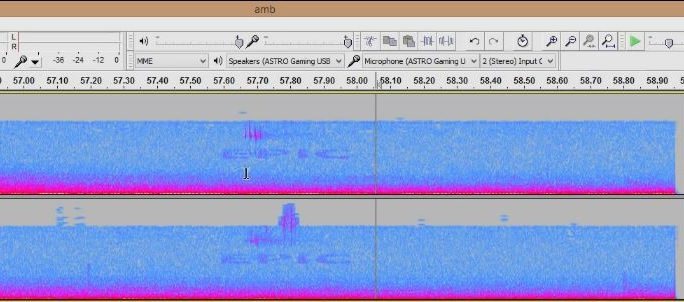
\includegraphics[width=7.7cm,keepaspectratio]{pics/audio_chapter/spectrogram_encoding.jpg}
    \caption{Message within the spectrogram viewed using Audacity.}
    \label{battlefield_spectrogram_easter_egg}
\end{figure}


\section{Waveform Audio (WAV)}
The Waveform Audio format commonly known as WAV is a popular file format for storing high quality digital audio files originally built by Microsoft. It bears many similarities to the PNG format in the internal structure/composition of the file: both begin with a very specific sequence of bytes (also known as the magic bytes) that help classification applications identify them, are separated into multiple parts (also known as chunks) that have their purpose and are extremely common in the modern day multimedia. WAV is one of the most common file formats that can be found in the digital world and that makes it a viable candidate for the message carrier role in the steganography domain. Like almost all other formats designed by Microsoft it has a few variations and extensions of the original specifier to accomodate more metadata or higher quality audio, but since they are much rarer than the simple and original standard, we will not focus on those altered versions in this thesis.

In the table below we can see the general structure of almost any WAV file that contains PCM data \footnote{PCM is an abbreviation for Pulse-code modulation which is the most common way of storing digitally the sampled analog audio signals.} which are basically the default option of every digital audio recording software. From the table we can notice how there aren't any metadata fields that are less important which could make for a good initial foothold in the steganography process.
\begin{center}
\begin{tabular}{|c|c|c|}
\hline
\textbf{Chunk field} & \textbf{Field Length} & \textbf{Description} \\ \hline
Chunk ID & 4 bytes & \begin{tabular}[c]{@{}c@{}}Always equal\\ to "RIFF"\end{tabular} \\ \hline
Chunk Size & 4 bytes & \begin{tabular}[c]{@{}c@{}}Length in bytes\\ of remaining file\end{tabular} \\ \hline
Format & 4 bytes & \begin{tabular}[c]{@{}c@{}}Always equal\\ to "WAVE"\end{tabular} \\ \hline
Subchunk ID & 4 bytes & \begin{tabular}[c]{@{}c@{}}Always equal \\ to "fmt "\end{tabular} \\ \hline
Subchunk size & 4 bytes & \begin{tabular}[c]{@{}c@{}}Always equal\\ to 16\end{tabular} \\ \hline
Audio Format & 2 bytes & Equal to 0x0001 \\ \hline
Nr. of channels & 2 bytes & \begin{tabular}[c]{@{}c@{}}Channel count\\ (1 mono, 2 stereo etc.)\end{tabular} \\ \hline
Sample Rate & 4 bytes & \begin{tabular}[c]{@{}c@{}}How many samples\\ per second(6000Hz,\\ 44100Hz, etc.)\end{tabular} \\ \hline
Byte Rate & 4 bytes & \begin{tabular}[c]{@{}c@{}}Product of SampleRate,\\ number of channels and\\ the byte per sample\\ (BitsPerSample/8)\end{tabular} \\ \hline
Block Align & 2 bytes & \begin{tabular}[c]{@{}c@{}}Actual byte count \\ for a full sample\\ (both channels in a \\ stereo file for example\\ result in 4 bytes for\\ a full sample)\end{tabular} \\ \hline
Bits Per Sample & 2 bytes & \begin{tabular}[c]{@{}c@{}}How many bits\\ in a sample for\\ a single channel\end{tabular} \\ \hline
Subchunk ID & 4 bytes & Equal to "data" \\ \hline
Subchunk size & 4 bytes & Length of actual data \\ \hline
Data & * & The actual data \\ \hline
\end{tabular}
\end{center}

However, we see a great deal of advantages as well based on the file structure:
\begin{itemize}
	\item \textbf{Uncompressed data} means that we do not have to go through the process of decompressing it, editing it, and then recompressing it in order to store any information. We are able to go sequentially through each byte and without being careless we can alter it in order  to perform least significant bit insertion and hide the message, making WAV a good carrier for any type of sequential steganography. There are a few issues that could arise, usually samples are stored on two bytes and altering the least significant bit of each byte will alter the associated sample in a much much greater way, so we must keep in mind the bit depth of the samples when inserting the data. Furthermore, we must be careful with the audio channels of the file since modifying only one channel will possibly introduce noise to the audio stream, raising red flags to intruders and blowing the cover of the carrier.
	\item \textbf{The chunked structure} of the format leads to the ability to insert custom chunks with our data because most parsers will simply ignore them and look for the relevant chunks that they need. There are also a few types of chunks such as INFO or JUNK that could be used for a safer and more covert communication because they are a part of the standard and that means there will be no risk of crashing the parser if they find a chunk they could not identify.
	\item \textbf{Length is known beforehand} means that we know where the audio data ends just by parsing a few relevant metadata fields. This means that it is very easy to compute the offset where the file ends and we can begin embedding secrets while avoiding breaking the parsers or disturbing the audio data.
\end{itemize}

In conclusion, WAV is an impressive carrier format worthy of being used in the steganography process due to the fact that it is commonly seen on the Internet, has no compression that can affect the secret message and can easily work with all the algorithms presented over the course of this thesis.

\section{The MPEG-1/2 Audio Layer III (MP3)}
Moving Pictures Experts Group or MPEG for short has plenty of both official and unofficial standards, multiple versions etc. The focus of this subchapter will be on MPEG Versions 1 and 2 (the only officially accepted standards), or to be more precise, Layer III of these versions. As you can already see, there are tons of variations of what should  be a single and standardized format, but all of them exist for a good reason and have their own use cases, even though they differ in available bit rates or the sampling rate frequencies range. Talking about all of them would be pointless and would easily take hundreds of pages to showcase as they have been the result of many years of research and evolution, so instead we are going to focus on the most common standard that is available in the digital world, which is even more popular than the aforementioned audio file format, and that is MPEG Version 1 Layer 3, hereby known simply as MP3. While technically any version of the MPEG that uses Layer 3 is formally known as MP3, versions 2 and 2.5 are much rarer since they offer smaller bitrates and smaller frequency sampling rates, making them inadequate for audio usage in the modern day.

The biggest reason MP3 has been one of the most popular audio file formats used in the world since its invention back in 1993 is due to its ability to replay high quality audio samples while still keeping a very small disk usage overhead. It takes advantage of the Huffman coding to reduce the total length of the file, making it able to retain the same perceptible audio quality to the human ear while still compressing the final size between 75\% and 95\% of other uncompressed formats, such as WAV\cite{genesis_of_mp3}. However, due to the usage of compression algorithms, the long time the format was in development, the high number of standards and substandards and the inclusion of other formats in the same binary stream as the audio samples for various reasons, make the MP3 an incredibly complex format that need more advanced parsers than the ones found in other trivial formats, such as BMP or WAV.

Before beginning to talk about steganographic algorithms that could be applied to the format, we first need to understand the MP3 binary stream to make sure we do not alter bytes that could mark the file as corrupted, such as checksums or important headers. Nowadays, the structure of most MP3 files consists of two parts:
\begin{itemize}
	\item The \textbf{ID3} part, the metadata container where information such as the track artist, album name or even album art is stored.
	\item The actual \textbf{MP3} audio data, contains the audio samples in a special format.
\end{itemize}

ID3 is a standard used to store file metadata that is most commonly seen alongside MP3 files, which is why it is important to discuss it because it can offer a few interesting options that can be viable secret message carriers. It is always found at the beginning of the audio file such that any parsers that are not interested in the metadata will need to read only a few bytes in order to get the offset to the actual sound data. Similar to the PNG, it is a chunked structure that may contain multiple chunks (or frames as the standard specifies). We can see in table below the general structure of the ID3v2 header(the most common type of header, the previous versions being flagged as obsolete):

\begin{center}
\begin{tabular}{|c|c|}
\hline
\textbf{Chunk type}                                           & \textbf{Chunk size}                                       \\ \hline
\begin{tabular}[c]{@{}c@{}}Header\\ (REQUIRED)\end{tabular}   & 10 bytes                                                  \\ \hline
\begin{tabular}[c]{@{}c@{}}Extended Header\\ (OPTIONAL)\end{tabular} & \begin{tabular}[c]{@{}c@{}}Variable\\ Length\end{tabular} \\ \hline
\begin{tabular}[c]{@{}c@{}}Frames\\ (at least 1)\end{tabular} & \begin{tabular}[c]{@{}c@{}}Variable\\ Length\end{tabular} \\ \hline
\begin{tabular}[c]{@{}c@{}}Padding\\ (OPTIONAL)\end{tabular}  & \begin{tabular}[c]{@{}c@{}}Variable\\ Length\end{tabular} \\ \hline
\begin{tabular}[c]{@{}c@{}}FOOTER\\ (OPTIONAL)\end{tabular}   & 10 bytes                                                  \\ \hline
\end{tabular}
\end{center}

We can see from the table the similarities to other chunked file formats. Since modifying any of the important bytes from the header/footer or padding can lead to corrupted and unparsable files, we shall stray away from them. However the frames are a perfect environment for our messages since we can have almost any number of them (limited by the 4 bytes or 28 bits that form a synchsafe integer representing the total size of the ID3 header), along with a high range of official frame types that we can pick from that most parsers will probably ignore. We can see in the figure below a frame with the ID equal to APIC (short for attached picture) which is used to usually embed images into the stream that represent album art or covers.
\begin{figure}[H]
    \centering
    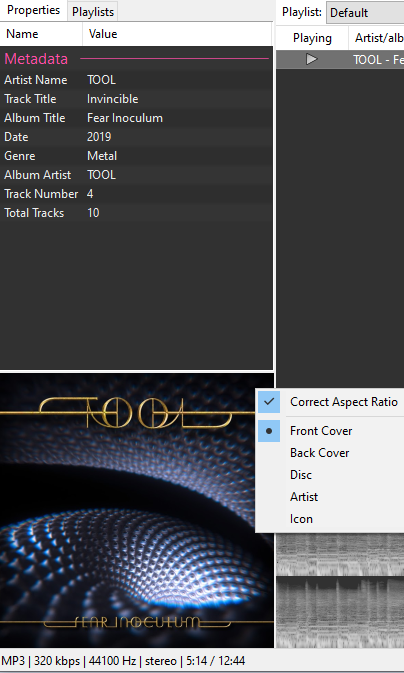
\includegraphics[height=8cm,keepaspectratio]{pics/audio_chapter/tool_cover_example.png}
    \caption{Front cover of the album Fear Inoculum by Tool}
\end{figure}

Our advantage is that there is no limit of frames with the ID equal to APIC there can be in a file so it is a prime target for metadata steganography when our message is a simple image. By changing a few bits we can mark the image as being the back cover of the song or we can even make it invalid such that it will exist in the binary stream but no renderers will show it. The process of parsing the metadata is simple after reading and understanding the documentation and results in a trivial encoding process. The difficult part is when attempting to write our image since it has to be inserted without breaking any of the other frames. After the entire process is done, we get something like this:
\begin{figure}[H]
    \centering
    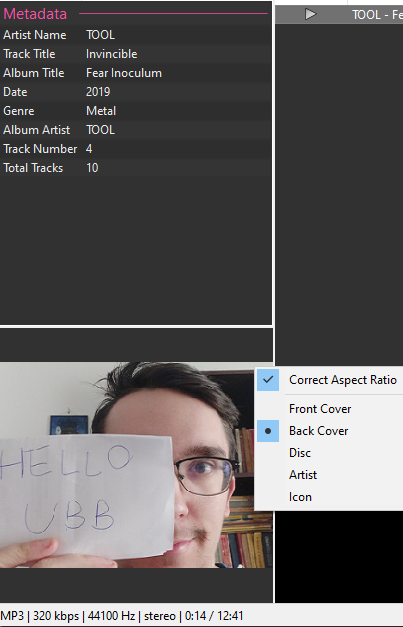
\includegraphics[height=8cm,keepaspectratio]{pics/audio_chapter/tool_backcover_example.png}
    \caption{Back cover which is our hidden image}
\end{figure}

Unfortunately, since MP3 is a much more complex format than we are accomodated with we will not look into the process of Least Significant Bit insertion as that would entitle too much trouble for such a simple result and since it is by default a compressed format it is not a significant loss because the available domain is smaller and we would not be able to achieve an acceptable performance. This is the reason why metadata and after-end steganography are the only viable methods when dealing with the MP3 file format.

In conclusion, MP3 is one of the best formats for metadata embedding since it has so many types of frames that are impossible to keep track of and that no user will possibly notice if they are not looking specifically for it. 
\end{multicols*}